% --------------------------------------------------------------
% This is all preamble stuff that you don't have to worry about.
% Head down to where it says "Start here"
% --------------------------------------------------------------
 
\documentclass[12pt]{article}
 
\usepackage[margin=1in]{geometry} 
\usepackage{mathtools}
\usepackage{bm}
\usepackage{subfig}

\setlength{\parskip}{1em}

% \newenvironment{theorem}[2][Theorem]{\begin{trivlist}
% \item[\hskip \labelsep {\bfseries #1}\hskip \labelsep {\bfseries #2.}]}{\end{trivlist}}
% \newenvironment{lemma}[2][Lemma]{\begin{trivlist}
% \item[\hskip \labelsep {\bfseries #1}\hskip \labelsep {\bfseries #2.}]}{\end{trivlist}}
% \newenvironment{exercise}[2][Exercise]{\begin{trivlist}
% \item[\hskip \labelsep {\bfseries #1}\hskip \labelsep {\bfseries #2.}]}{\end{trivlist}}
% \newenvironment{reflection}[2][Reflection]{\begin{trivlist}
% \item[\hskip \labelsep {\bfseries #1}\hskip \labelsep {\bfseries #2.}]}{\end{trivlist}}
% \newenvironment{proposition}[2][Proposition]{\begin{trivlist}
% \item[\hskip \labelsep {\bfseries #1}\hskip \labelsep {\bfseries #2.}]}{\end{trivlist}}
% \newenvironment{corollary}[2][Corollary]{\begin{trivlist}
% \item[\hskip \labelsep {\bfseries #1}\hskip \labelsep {\bfseries #2.}]}{\end{trivlist}}
\newenvironment{question}[2][Question]{\begin{trivlist}
\kern10pt
\item[\hskip \labelsep {\bfseries #1}\hskip \labelsep {\bfseries #2.}]}{\end{trivlist}}


\newcommand\TODO[1]{\textcolor{red}{#1}}

\begin{document}
 
% --------------------------------------------------------------
%                         Start here
% --------------------------------------------------------------
 
%\renewcommand{\qedsymbol}{\filledbox}
 
\title{DD2434 Machine Learning, Advanced Course Assignment 1}
\author{Lin Chun Hung, chlin3@kth.se} 
 
\maketitle


% Question 1
\begin{question}{1}
% TODO: Fix the arguments
Consider input output pairs are linked by the mapping to have the following
 relation:
$$ 
    \bf{t}_i = f(\bf{x}_i) + \bm{\epsilon}
$$
where the $\bm{\epsilon}$ is the unbiased random noise. Since we have no piror knowledge
on the random noise term, the random noise is then assumed as following the normal
distribution. TODO: More on this \par

With the assumption that features are uncorrelated, we choose the spherical
covariance matrix for the likelihood.
\end{question}
% End question 2



% Question 2
\begin{question}{2}
Consider the general product rule of probability:
$$\mathrm {P} \left(\bigcap _{k=1}^{n}A_{k}\right)=
  \prod _{k=1}^{n}\mathrm {P} \left(A_{k}\,{\Bigg |}\,\bigcap _{j=1}^{k-1}A_{j}\right)$$

Therefore the likelihood would be:
$$ 
  p(\bf{T}\mid f,\bf{X}) =
  \prod _{i=1}^{N}p(\bf{t}_i \mid \bf{t}_{i-1},...,\bf{t}_{1},
  f,\bf{X})
$$

\end{question} 
% End question 2


% Question 3 
\begin{question}{3}

$$ 
  p(\bf{T}\mid \bf{X},\bf{W}) =
  \prod _{i=1}^{N}N(\bf{W}\bf{x}_i, \sigma^2\bf{I})
$$

\end{question}
% End question 3

% Question 4
\begin{question}{4}
The choice of piror distribution reflects the choice of regularizer. Chossing L1 
norm as regularizer is known as the lasso (least absolute shrinkage and selection operator).
The regularizer will force some weighting coefficients $w_j$ to be zero, given 
a proper choice of model parameter $\tau$. It plays the role of feature selection
since those zero weighting coefficients indicate that the corresponding features
are irrelvant to the output. \par

The penalization term or the negative log-prior:
$$  \frac{\lambda}{2} \left \|\textbf{vec}(\bf{W} - \bf{W}_0)\right \|_{q}  $$

\begin{figure}[h!]
  \centering
  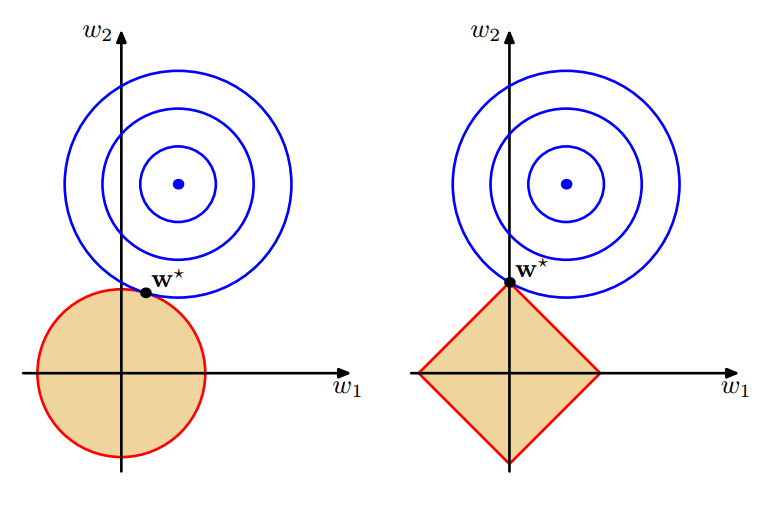
\includegraphics[width=0.5\linewidth]{q4_regular.png}
  \caption{A boat.}
  \label{fig:boat1}
\end{figure}

TODO: Discussion
\end{question}
% End question 4



% Question 5
\begin{question}{5}
TODO: Add dimension\\
Consider the regression equation in general:
$$\textbf{T} = \textbf{WX} + \textbf{ErrorMatrix} $$
Therefore, the likelihood in terms of matrix normal distribution is:
\begin{align*}
p(\bf{T}\mid \bf{X}, \bf{W}) &= 
  \mathcal{MN}_{D \times N}(\bf{WX}, \bf{I}, \sigma^2 \bf{I}) \\ 
  &= \mathcal{N}_{DN}(\bf{vec}(\bf{WX}), \sigma^2 \bf{I})
\end{align*}
The prior is:
\begin{align*}
p(\bf{W}) &= 
  \mathcal{MN}_{D \times q}(\textbf{W}_0, \bf{I}, \tau^2 \bf{I}) \\
  &= \mathcal{N}_{Dq}(\textbf{vec}(\textbf{W}_0), \tau^2 \bf{I})
\end{align*}

Due to the choice of a conjugate Gaussian prior distribution, the posterior will 
also be Gaussian:
$$
p(\textbf{W}\mid \textbf{X}, \textbf{T}) =
  \mathcal{N}_{Dq}(\textbf{vec}(\textbf{W}_{p0}), \bm{\Sigma}_{p0} )
$$

To calculate the mean and covariance of the posterior over the parameters,
Consider the equation 7 in the question with respect to the parameters $\textbf{W}$
 and compare the quadratic and linear terms of the exponents in both sides:
\begin{align*}
  p(\textbf{W}\mid \textbf{X}, \textbf{T}) =&
  \frac{1}{Z}p(\textbf{T}\mid \textbf{X}, \textbf{W})p(\textbf{W})  \\
  \ln p(\textbf{W}\mid \textbf{X}, \textbf{T}) =&
  \ln p(\textbf{T}\mid \textbf{X}, \textbf{W}) + \ln p(\textbf{W}) + \text{Const.} \\
\end{align*}
\begin{align*}
  LHS =& -\frac12[\textbf{vec}(\textbf{W}) - \textbf{vec}(\textbf{W}_{p0)}]^T
          \bm{\Sigma}_{p0}^{-1}[\textbf{vec}(\textbf{W})-\textbf{vec}(\textbf{W}_{p0})] \\
  RHS =& -\frac{1}{2\sigma^2}[\textbf{vec}(\textbf{T}) - \textbf{vec}(\textbf{WX})]^T
                             [\textbf{vec}(\textbf{T}) - \textbf{vec}(\textbf{WX})] \\
       &-\frac{1}{2\tau^2}[\textbf{vec}(\textbf{W}) - \textbf{vec}(\textbf{W}_0)]^T
                          [\textbf{vec}(\textbf{W}) - \textbf{vec}(\textbf{W}_0)]
\end{align*}

Consider the quadratic terms on both sides:
\begin{equation} \label{eq:q5-covar}
  \begin{aligned}[b]
    -\frac12\textbf{vec}(\textbf{W})^T\bm{\Sigma}_{p0}^{-1}\textbf{vec}(\textbf{W})
    =& -\frac{1}{2\sigma^2}\textbf{vec}(\textbf{WX})^T\textbf{vec}(\textbf{WX})
    -\frac{1}{2\tau^2}\textbf{vec}(\textbf{W})^T\textbf{vec}(\textbf{W}) \\
    -\frac12\textbf{vec}(\textbf{W})^T\bm{\Sigma}_{p0}^{-1}\textbf{vec}(\textbf{W})
    =& -\frac{1}{2\sigma^2}\textbf{vec}(\textbf{W})^T(\mathbf{X}^T \otimes \mathbf{I}_D)^T
    (\mathbf{X}^T \otimes \mathbf{I}_D)\textbf{vec}(\textbf{W}) \\
    & -\frac{1}{2\tau^2}\textbf{vec}(\textbf{W})^T\textbf{vec}(\textbf{W}) \\
    -\frac12\bm{\Sigma}_{p0}^{-1} =&
    -\frac{1}{2\sigma^2}(\mathbf{X} \otimes \mathbf{I}_D)(\mathbf{X}^T \otimes \mathbf{I}_D) 
    -\frac{1}{2\tau^2} \mathbf{I}_{Dq}\\
    \bm{\Sigma}_{p0}^{-1} =& \hspace{5mm} 
    \frac{1}{\sigma^2}(\mathbf{X}\mathbf{X}^T)\otimes \mathbf{I}_D +\frac{1}{\tau^2}\mathbf{I}_{Dq}
  \end{aligned}
\end{equation}

Consider the linear terms on both sides:  
\begin{align*}
    \textbf{vec}(\textbf{W})^T\bm{\Sigma}_{p0}^{-1}\textbf{vec}(\textbf{W}_{p0})
    =& \hspace{1mm} 
       \frac{1}{\sigma^2}\textbf{vec}(\textbf{WX})^T\textbf{vec}(\textbf{T}) 
     + \frac{1}{\tau^2}\textbf{vec}(\textbf{W})^T\textbf{vec}(\textbf{W}_0)\\
    \textbf{vec}(\textbf{W})^T\bm{\Sigma}_{p0}^{-1}\textbf{vec}(\textbf{W}_{p0})
    =& \hspace{1mm} 
       \frac{1}{\sigma^2}\textbf{vec}(\textbf{W})^T(\mathbf{X}\otimes\mathbf{I}_D)
       \textbf{vec}(\textbf{T}) 
     + \frac{1}{\tau^2}\textbf{vec}(\textbf{W})^T\textbf{vec}(\textbf{W}_0)\\
    \textbf{vec}(\textbf{W}_{p0}) =& \hspace{1mm} 
       \bm{\Sigma}_{p0}[\frac{1}{\sigma^2}(\mathbf{X}\otimes\mathbf{I}_D)
       \textbf{vec}(\textbf{T}) + \frac{1}{\tau^2}\textbf{vec}(\textbf{W}_0)] \\
\end{align*}
\begin{equation} \label{eq:q5-mean}
    \textbf{vec}(\textbf{W}_{p0}) =
    [\frac{1}{\sigma^2}(\mathbf{X}\mathbf{X}^T)\otimes \mathbf{I}_D +\frac{1}{\tau^2}\mathbf{I}_{Dq}]^{-1}
       [\frac{1}{\sigma^2}(\mathbf{X}\otimes\mathbf{I}_D)
       \textbf{vec}(\textbf{T}) + \frac{1}{\tau^2}\textbf{vec}(\textbf{W}_0)]
\end{equation}

Consider an infinitely broad prior, which means $\tau \to \infty$, reduces the 
mean and covariance of the posterior to the mean and covariance of the likelihood
estimated under maximum likelihood approach. \par

The constant $Z$ plays no role in the calculation since only the quadratic and linear
 terms are considered.
% Subsitute back \eqref{eq:q5-covar} and \eqref{eq:q5-mean} into the posterior

\end{question}
% End question 5

% Question 6
\begin{question}{6}
The marginal distribution of $\mathbf{t}$ is given by:
\begin{equation}
  Bitshop 6.61
\end{equation}
where the covariance matrix C has elements:
\begin{equation}
  Bitshop 6.62
\end{equation}

The prior tells how two points in the data set are similar with the choice of the
kernal. As the result, the ouputs of the underlying function of the corresponding
two points will be more strongly correlated than dissimilar points. 

From the marginal distribution of $\mathbf{t}$, we can see that the covariance
matrix consists of two components: the covariance of the prior and the variance of
the noise. Notes that the noise are assumpted as independent among data points.

For simplicity, we choose the mean vector of prior to zero vector. It is because
we have no prior knowledge of the distribution of the instaniation of functions or
the distribution of functions in function-space view.

TODO: Add graph 
\end{question}
% --------------------------------------------------------------
%     You don't have to mess with anything below this line.
% --------------------------------------------------------------
%-----------------------------------
% \begin{equation} \label{eq:constantspeed}
%   v=\frac{s}{t}
%   \end{equation}
%-----------------------------------
% It is very important to remember that Equation~\eqref{eq:constantspeed} only works for   objects moving at \emph{constant speed}. This reference uses the \verb|\eqref{eq:constantspeed}| feature offered by \verb|amsmath| package.

\end{document}
